\chapter{Chapter 1: Introduction}
\section{Background}
In recent years, Kubernetes has emerged as the de facto standard for container orchestration, revolutionizing the way modern applications are deployed and managed \cite{google-no-date}. 
Organizations are incresingly adopting containerized workloads to leverage their multiple benefits, including scalability, portability, and efficiency in managing microservices architectures.
Kubernetes provides a robust framework for orchestrating these workloads, ensuring automated deployment, scaling, and operation of such workloads in a highly resilient manner. 

Despite the myriad of benefits that Kubernetes offers, the setup, and management of a Kubernetes cluster can often be complex and extremely time-consuming. The deployment
process involves provisioning infrastructure, configuring networking, setting up security rules, and configuring various add-ons, all of which require expertise and manual effort. For 
organizations and developers looking to ship quickly, this complexity introduces delays in application deployment, and reduces team velocity.

The traditional approach to deploying a containerised application and provisioning Kubernetes clusters in the cloud often involves multiple steps, including managing cloud provider integrations, and 
a lot of configuration. This process can take hours, or even days, depending on the use case, and the specific configuration required. As businesses demand quicker iteration cycles and seamless
cloud integration, there is a growing need for simplified, automated provisioning solutions that reduce setup time and eliminate operational friction.

As such, for this final year project, I have decided to build \texttt{cloudkube}, which steamlines the provisioning of Kubernetes clusters in the cloud, enabling users to spin up fully
configured clusters in the cloud within minutes. By abstracting away the complexities of infrastructure management, \texttt{cloudkube} allows developers to focus on deploying applications rather 
than managing the underlying infrastructure. This report explores the design, implementation, and impact of \texttt{cloudkube} in accelerating Kubernetes adoption while maintaining the flexibility
and robustness required for production grade deployments.




\section{Objective}
The main objective of this project was to speed up the turnaround time for deployment of new SpeechLab applications. The main idea of this tool is to abstract away in-depth knowledge of cloud technologies from researchers, and allow them to readily and easily deploy their ASR applications to the cloud at the press of a button. This will allow researchers to then concentrate their efforts on the development of the ML model in the ASR application, and not have to worry about low-level cloud implementation details such as creating a security group role to allow ingress/egress traffic, or configuring their local environment to hit the cluster.  

Drawing inspiration from minikube, which is a quick way to spin up a local cluster, for this FYP, I have decided to build \texttt{cloudkube}, which quickly spins up a Kubernetes cluster in the  cloud. Users then have a simple barebones Kubernetes cluster hosted in the cloud where they can do dev testing. 

The functional requirements for this project are detailed as follows:
\vspace{-1em} % Adjust vertical space here
\begin{enumerate}[label=\alph*., itemsep=0pt]
    \item \texttt{cloudkube} should provision infrastructure such as compute instances, storage, networking, and Kubernetes clusters in the cloud.
    \item \texttt{cloudkube} should be easily extendable to different cloud providers.
    \item \texttt{cloudkube} should create a Kubernetes environment, including deploying essential components like ingress controllers.
    \item \texttt{cloudkube} should allow users to easily deploy containerized ASR applications to the Kubernetes cluster.
    \item \texttt{cloudkube} should be able to deprovision and clean up resources without leaving anything dangling to prevent unnecessary costs.
    \item \texttt{cloudkube} should maintain the state of provisioned infrastructure to avoid dangling resources in the cloud.
\end{enumerate}
The non-functional requirements for this project are detailed as follows:
\vspace{-1em} % Adjust vertical space as needed

\begin{enumerate}[label=\alph*., itemsep=0pt]
    \item \texttt{cloudkube} should be easy to use, and have a gentle learning curve.
    \item \texttt{cloudkube} should be user-friendly, with clear command structures and help options.
    \item \texttt{cloudkube}, the CLI tool, should provision resources and deploy applications within a reasonable time frame.
    \item \texttt{cloudkube} should provision and deprovision resources idempotently and atomically.
    \item \texttt{cloudkube} should be able to work across different environments, including Windows, MacOS, and Linux.
    \item \texttt{cloudkube} should support the addition of new features or integrations.
\end{enumerate}

\section{Project Scope}

The scope of this project is focused on building a minimum viable project for \texttt{cloudkube}, to provision infrastructure for hosting applications in a Kubernetes environment in the cloud. \texttt{cloudkube} aims to simplify the development process by automatic infrastructure provisioning, Kubernetes cluster setup, cloud configuration, as well as application deployment. While the potential of \texttt{cloudkube} is massive, with possibilities for features such as multi-cloud support, advanced monitoring integrations, extensibility of modules and infrastructure templates, the scope of this project has been deliberately constrained due to the time frame of this FYP.  

Given the limited time frame, this project focuses on delivering core functionalities, which are as follows:

\vspace{-1em} % Adjust vertical space as needed

\begin{enumerate}[label=\alph*., itemsep=0pt]
    \item Efficiently spin up a Kubernetes cluster that applications can be easily deployed to.
    \item Allow some customizability of the infrastructure:
    \vspace{-0.5em}
    \begin{enumerate}[label=\roman*., itemsep=0pt]
        \item Architecture of compute instances.
        \item Use of ingress controller.
        \item Use of elastic file system for persistent volumes functionality in Kubernetes.
    \end{enumerate}
    \item State tracking to ensure idempotent and consistent behavior.
    \item Configuration of local environment to communicate with the Kubernetes cluster.
    \item Clean deprovisioning and tear down of resources.
\end{enumerate}

\section{Contributions}
This section highlights the key contributions made during the course of this project. The key contributions to this project can be roughly broken down into two parts. 
The first and main part relates to the infrastructure provisioning, which allows for any containerised workload to be deployed to a Kubernetes cluster hosted on the AWS cloud. 
The second part relates to optimizing the deployment of the ASR application. While the initial scope of this FYP was to provision infrastructure
for SpeechLab applications, this FYP has gone beyond this goal, and \texttt{cloudkube} has proved to be scalable, and extendable to different
types of Kubernetes workloads.

\textbf{Contributions toward Infrastructure Provisioning Workflow}
\vspace{-1em}
\begin{enumerate}[label=\alph*., itemsep=0pt]
    \item \textbf{Optimized the workflow for creating Kubernetes clusters in the cloud:} In order to facilitate creating Kubernetes clusters in the cloud, I developed the \texttt{cloudkube} CLI tool to automate the provisioning of Kubernetes clusters, as well as their corresponding dependencies in the cloud.
    \item \textbf{Creation of a user-friendly interface:} \texttt{cloudkube} was created with clear command structures and help options to ensure ease of use. As a tool aimed at developers who are not experts in cloud, \texttt{cloudkube} was built to abstract away in-depth cloud intricacies.
    \item \textbf{Idempotency and Atomic Provisioning:} To align with the requirements stated above, \texttt{cloudkube} was also developed with state tracking, to ensure idempotent and atomic provisioning and deprovisioning of resources to prevent resource leaks and unnecessary costs.
    \item \textbf{Easy user configurability:} After speaking to developers working on SpeechLab applications, and noting the use cases of different Kubernetes workloads, \texttt{cloudkube} provides customization options for infrastructure components such as compute instances, ingress controllers, and persistent volumes.
    \item \textbf{Optimization of development workflow for authenticating local machine with Kubernetes cluster:} \texttt{cloudkube} also facilitates the configuration of local environments to communicate and authenticate seamlessly with the Kubernetes cluster.
    \item \textbf{Extensive testing: } Extensive testing was also conducted to ensure the reliability and performance of the \texttt{cloudkube} tool. This included running multiple Kubernetes workloads against the provisioned cluster, which will be explained in detail in Chapter 5.
\end{enumerate}

\textbf{Contributions toward Optimizing ASR Kubernetes Deployment}
\vspace{-1em}
\begin{enumerate}[label=\alph*., itemsep=0pt]
    \item \textbf{Optimized workflow for copying of models into compute worker instances:} The previous workflow for copying of the models into the EC2 worker instances was via secure copy \texttt{scp}. In this project, a more streamlined process was developed, and models were automatically pulled from cloud storage into compute instances \cite{song-yu-2023}.  
\end{enumerate}
\newpage
% \section{Project Schedule}
% The project schedule is presented in Table \ref{table:project_schedule}. A Gantt chart for the project schedule is shown in Figure \ref{fig:gantt_chart}. It should be noted that these start and end dates serve as rough guidelines, especially for the implementation phase of the project.
% \ref{table:project_schedule}

% \begin{table}[h!]
% \centering
% \begin{tabular}{|c|l|c|c|}
% \hline
% \textbf{Index} & \textbf{Task Name} & \textbf{Start Date} & \textbf{End Date} \\ \hline
% \multicolumn{4}{|c|}{\textbf{Preparation Phase}} \\ \hline
% 1 & Literature Review & 31 May 2024 & 30 Jul 2024 \\ \hline
% 2 & Requirements Analysis & 14 Jun 2024 & 15 Jul 2024 \\ \hline
% 3 & Requirements Refinement & 15 Jul 2024 & 30 Jul 2024 \\ \hline
% 4 & System Design Development and Refinement & 15 Jul 2024 & 30 Sept 2024 \\ \hline
% \multicolumn{4}{|c|}{\textbf{Implementation Phase}} \\ \hline
% 5 & Optimizing ASR Kubernetes Deployment & 1 Oct 2024 & 7 Oct 2024 \\ \hline
% 6 & Provisioning Infrastructure for ASR & 7 Oct 2024 & 9 Oct 2024 \\ \hline
% 7 & Development of main CLI interface of \texttt{cloudkube} & 1 Oct 2024 & 31 Oct 2024 \\ \hline
% 8 & Ingress Controller Implementation & 1 Nov 2024 & 15 Nov 2024 \\ \hline
% 9 & Persistent Volumes Implementation & 15 Nov 2024 & 29 Nov 2024 \\ \hline
% 10 & \texttt{cloudkube} interactive setup wizard & 15 Nov 2024 & 29 Nov 2024 \\ \hline
% 11 & \texttt{cloudkube} commands setup & 2 Dec 2024 & 16 Dec 2024 \\ \hline
% \multicolumn{4}{|c|}{\textbf{Testing Phase}} \\ \hline
% 12 & ASR Kubernetes Workload & 16 Dec 2024 & 15 Jan 2025 \\ \hline
% 13 & Multi Service Kubernetes Workload & 16 Dec 2024 & 15 Jan 2025 \\ \hline
% \multicolumn{4}{|c|}{\textbf{Documentation Phase}} \\ \hline
% 14 & Project Proposal & 12 Aug 2024 & 2 Sept 2024 \\ \hline
% 15 & Interim Report & 16 Dec 2024 & 30 Jan 2025 \\ \hline
% 16 & Final Report & 30 Jan 2025 & 24 Mar 2025 \\ \hline
% 17 & Presentation & 24 Mar 2025 & 14 May 2025 \\ \hline
% \end{tabular}
% \caption{Project Schedule}
% \label{table:project_schedule}
% \end{table}

% \begin{figure}[h!]
%     \centering
%     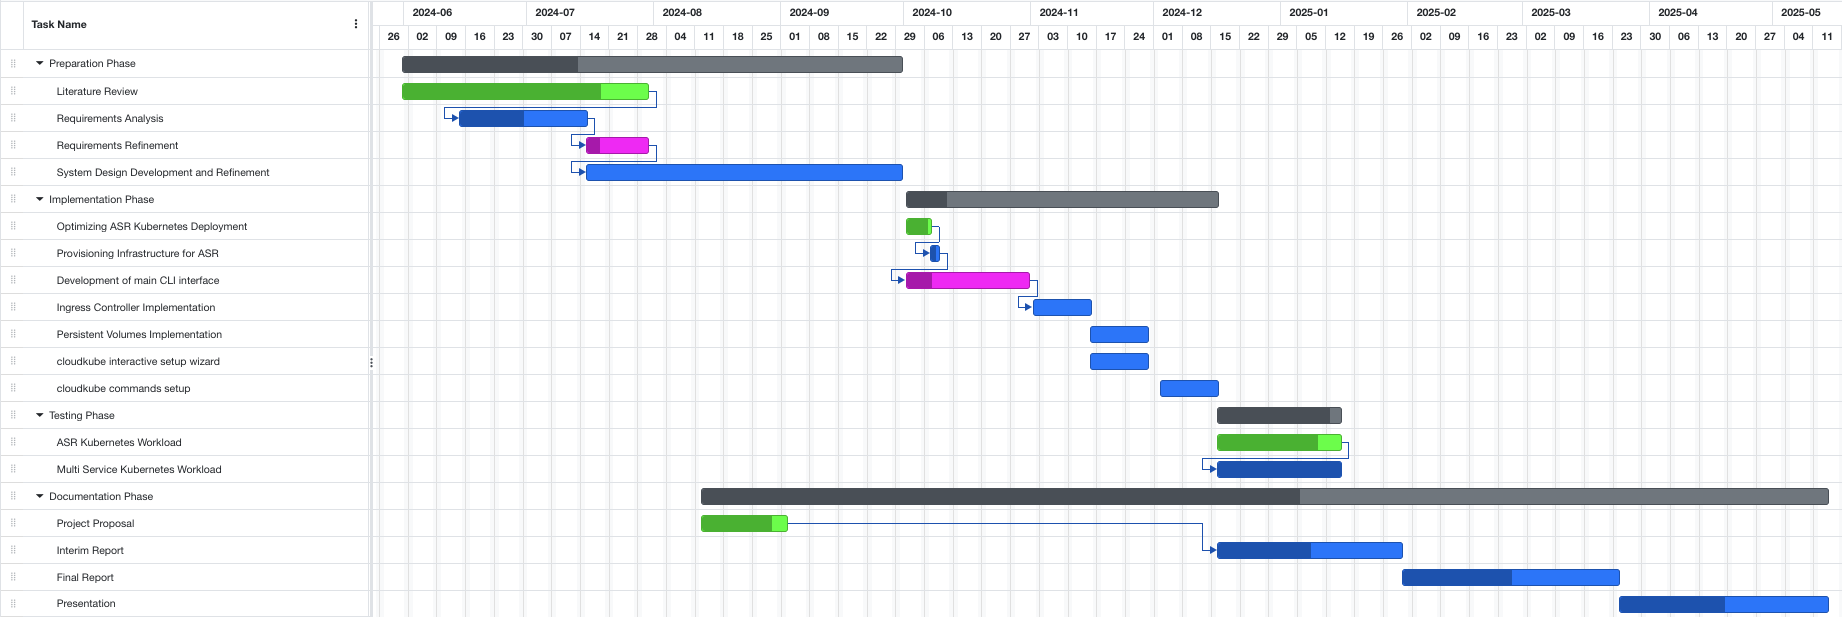
\includegraphics[width=\textwidth]{fig/gantt_chart.png}
%     \caption{Gantt Chart for Project Schedule}
%     \label{fig:gantt_chart}
% \end{figure}

\section{Report Organisation}
This report is structured into 5 different chapters, each detailing different aspects of the project.

\textbf{Chapter 1 - Introduction: } This chapter presents the background and introduction of the project. In this chapter, I elucidate some of the motivations for this project, and a brief overview on the intended outcome of this project.

\textbf{Chapter 2 - Literature Review: } This chapter reviews relevant technologies, and builds a foundational understanding for technical terminology used in future chapters. For completeness, this chapter will also discuss some of the pros and cons of each technology, which become relevant in later chapters.

\textbf{Chapter 3 - Planning and Design: } This chapter focuses on the analysis and design of the proposed solutions. In this chapter, I explore the current methods for handling containerised workloads, and show an optimized workflow for my proposed application.

\textbf{Chapter 4 - Implementation: } This chapter delves into the implementation of the proposed solutions. In this chapter, I detail the code and architecture used for \texttt{cloudkube}.

\textbf{Chapter 5 - Results and Analysis: } This chapter discusses the results of my proposed application, \texttt{cloudkube}. In this chapter, we will see the deployment of two applications to a Kubernetes environment provisioned by \texttt{cloudkube} - (1) ASR Application, and (2) Multi-service Kubernetes Application.

\textbf{Chapter 6 - Conclusion and Future Work: } This chapter presents the conclusions and recommendations for future work. 